\cotefile{68}
\scanpage{33}
\[
\left\{\begin{aligned}
G\cap(C\setminus C_0)&=G^{\unsure{\times|\ast}}\\
P\cap(C\setminus C_0)&=P^{\ast}\\
C\setminus(G\cup P)&=N\quad\text{(positions nulles, i.e. gagnantes}\\
&\hphantom{=N\quad}\text{pour aucun des deux joueurs)}
\end{aligned}\right.
\]

\unsure{Une|Les} position $x$ \unsure{sera|seront} encore dite \uline{gagnante} (resp. \uline{perdante}) si $x\in G$ (resp. $x\in P$) — cette terminologie coïncide avec la précédente si $x\notin C_0$. On aura, posant
\[
\begin{aligned}
&\deleted{\unsure{G(j)=\{x\in}}\\
&\widehat C(j)=\{x\in C\mid\widehat\alpha(x)=j\}
\end{aligned}
\]
(de sorte que $C$ apparaît comme réunion disjointe des deux ens. $\widehat C(j)$, $j\in J$),
\[
\left\{\begin{aligned}
G(j)\cap\widehat C(j)&=\deleted{\unsure{\{x\in}}\widehat C(j)\cap G\\
G(j)\cap\widehat C(\bar j)&=\widehat C(\bar j)\cap P
\end{aligned}\right.
\]
donc \inserted{les} $G(j)$ $(j\in J)$ se réconstituent à partir de $\widehat\alpha$ et des ensembles $G$, $P$.

On aura, pour $x\in C\setminus C_0$
\[
\begin{aligned}
x\in G&\Longleftrightarrow\exists\, y\in R(x)\ \inserted{\text{tel que}}\ y\in P
&&\text{i.e.}\quad R(x)\cap P\ne\varnothing\\
x\in P&\Longleftrightarrow\forall\, y\in R(x),\ \text{on a}\ y\in G
&&\text{i.e.}\quad R(x)\unsure{\subset|\in}G
\end{aligned}
\]
i.e.
\[
\begin{aligned}
G\cap(C\setminus C_0)\deleted{\unsure{\cap G|G}}&=\{x\in C\setminus C_0\mid R(x)\cap P\ne\varnothing\}\\
P\cap(C\setminus C_0)&=\{x\in C\setminus C_0\mid R(x)\subset G\}
\end{aligned}
\]
% archive sheet number: 32

\scanpage{34}
\uline{Proposition} Soit\deleted{\unsure{ent}} $(C,R,J,\widehat\alpha,G_0:J\longrightarrow\unsure{\mathcal P|\mathfrak P|\mathscr P}(C_0))$ un jeu de positions à deux joueurs jouant alternativement, $G\subset C$ et $P\subset C$, l'ens des positions gagnantes resp. perdantes. Soient $\widetilde G,\widetilde P$ deux parties de $C$ ayant les propriétés suivantes
\[
\begin{aligned}
1)\quad &\forall x\in\widetilde G,\quad\exists\,y\in R(x)\quad\text{tel que}\quad y\in\widetilde P\\
2)\quad &\forall x\in\widetilde P,\quad\deleted{\unsure{\exists}}\forall\,y\in R(x),\quad\text{on a}\quad y\in\widetilde G\\
3)\quad &\forall x\in\widetilde G\cap C_0,\ \text{on a}\quad x\in G_0(\widehat\alpha(x))\\
4)\quad &\forall x\in\widetilde P\cap C_0,\ \text{on a}\quad x\in G_0(\overline{\widehat\alpha}(x))
\end{aligned}
\]
Alors, si dans $C$ il n'existe pas de \deleted{\unsure{jeu}}\inserted{partie} infinie, on a
\[
\widetilde G\subset G,\qquad\widetilde P\subset P
\]
Si de plus on suppose \deleted{\unsure{la} réunion disjointe des deux parties $G_0(j)$ $(j\in J)$, alors on a} \inserted{que $\widetilde G$ et $\widetilde P$ sont complémentaires} l'un de l'\deleted{$\unsure{\widetilde G}$}autre, \deleted{\unsure{donc} $G$} et $G_0(j)\cap G_0(\bar j)=\varnothing$ (donc $G\cap P=\varnothing$) alors on a $\widetilde G=G$, $\widetilde P=P$ (et par suite $G\cup P=C$ donc $G_0(j)\cup G_0(j')=C_0$)

\uline{Cor} Soit $(C;-)$ un jeu alterné tel que \deleted{\unsure{$G_0(j)$ et}}

a) Pas de partie infinie \qquad b) $C_0$ réunion disjointe des $G_0(j)$ et $G_0(\bar j)$. Soient $\widetilde G,\widetilde P$ deux parties de $C$. Pour que \deleted{\unsure{$G$}}l'on ait $\widetilde G=G$, $\widetilde P=P$, il f et s. que $\widetilde G$ et $\widetilde P$ soient complémentaires l'un de l'autre, et satisfassent les conditions 1) à 4) ci-dessus.
% archive sheet number: 33

\scanpage{36}
\uline{Exponentielle} (en car. 0)

\deleted{\unsure{I)}} \inserted{I) \uline{généralités}}

$\deleted{U}A$ $\mathbb Q$-algèbre (ass. avec 1)

$N(\deleted{U}A)$ ens des él. nilp. de $\deleted{U}A$. On a donc $1+N(\deleted{U}A)\subset\deleted{U}A^*$ (ens des él. inv. de $\deleted{U}A$)
\[
N(\deleted{U}A)\xrightarrow{\exp}1+N(\deleted{U}A)\qquad
\exp x=\sum_{n\geq0}\frac{x^n}{n!}
\]
\uline{Th 1} 1) $\exp$ est bijective. L'application inverse est donnée par
\[
\log(1+y)=\sum_{n\geq1}(-1)^{n+1}\frac{y^n}{n}\qquad(y\in N(\deleted{U}A))
\]
2) Si $x,y\in N(\deleted{U}A)$ commutent, alors $x+y\in N(\deleted{U}A)$ et
\[
\exp(x+y)=\exp x\ \exp y
\]
\margin{NB $\exp 0=1$}
Si $u,v\in 1+N(\deleted{U}A)$ commutent, alors $uv\in 1+N(\deleted{U}A)$, et
\[
\log(uv)=\log u+\log v
\]
\margin{NB $\exp 1=0$}
3) Soit $L\subset\deleted{U}A$ un sous-$\mathbb Q$-espace vectoriel tel que $x\in L$, $n\in\mathbb N^*$ implique $x^n\in L$, \deleted{Alors} et $L$ formé d'éléments nilpotents. Alors
\[
x\mathrel{\unsure{\mapstochar\relbar|\mapsto}}\exp x:\quad L\xrightarrow{\sim}1+L
\]
\uline{Remarque} Soit \deleted{les conditions de 3), supposons que} \inserted{$L\subset\deleted{U}A$ un sous $\mathbb Q$-espace vectoriel de $A$} tel que $L\subset N(A)$, et tel que $x,y\in L\ \Rightarrow xy\in L$. Alors $L\xrightarrow{\sim}1+L$ par 3°, et de plus $1+L$ est un sous-groupe de $\deleted{U}A^*$. D'où par transport de str. une str. de groupe sur $L$. Elle est comm. \unsure{ssi} $L$ est commutatif, i.e. \unsure{si|ssi} $x,y\in L\Rightarrow xy=yx$ — \inserted{et dans ce cas cette structure est l'\uline{addition} de $L$.}
% slanted
\margin{réciproque? par \unsure{introduction} d'indéterminées --}

\uline{Exemple 1} Soient $K$ une $\mathbb Q$-alg. comm., $\deleted{U}A$ une $K$-algèbre (ass. avec 1), $J$ un \deleted{\unsure{fini|formé}}\inserted{nil}idéal de $K$. Alors $J.\deleted{U}A$ satisfait les conditions de la Remarque, et on a donc
\[
J\deleted{U}A\longrightarrow 1+J\deleted{U}A
\]
\uline{NB} Soient $K_0=K/J$, $\deleted{U}A_0=\deleted{U}A/J\unsure{AU|\deleted{U}A|\mathbb A}=\deleted{U}A\otimes_K K_0$, \inserted{$\unsure{a|\alpha}_{\unsure{U|u}}:\deleted{U}A\to\deleted{U}A_0$ app. can.} Alors \deleted{$JA\unsure{{}={}|{}\to{}|\mathrm{est}}$}
\[
J\deleted{U}A=\{x\in\deleted{U}A\mid\alpha_U(x)=0\},\qquad
1+J\deleted{U}A=\{x\in\deleted{U}A\mid\alpha_U(x)=1\}
\]

\uline{Exemple 2} $K,J$ comme dans Exemple 1, \inserted{mais \unsure{avec|ici} $J$ nilpotent,} $M$ un $K$-module, $U=\operatorname{End}_K(M)$, \deleted{$\unsure{U_0=U\otimes_K K_0=U/JU|M_0=M\otimes_K K_0=M/JM}$}\inserted{$M_0=M\otimes_K K_0\simeq M/\deleted{\otimes}JM$}, \deleted{$\unsure{L=}$}$\alpha_M:M\to M_0$ appl. can.; posons \inserted{alors}
\[
L=\{u\in U:\operatorname{End}_K(M)\mid u\otimes_K K_0=0\}
=\{\unsure{u\in U|u\in M|u}\mid u(M)\subset JM\}
\]
\[
1+L=\{u\in U=\operatorname{End}_K(M)\mid u\otimes_K K_0=\mathrm{id}_{M_0}\}.
\quad\deleted{\text{Ceci posé,}}
\]
Ceci posé, les conditions de la remarque sont satisfaites, donc on a $\exp:L\xrightarrow{\sim}1+L$.
% archive sheet number: 35

\scanpage{37}
II) Groupes à un paramètre formels

$K$ $\mathbb Q$-algèbre comm. unifère.

$\overline{\mathbb G}_{aK}$ droite formelle sur $K$ $\bigl(\overline{\mathbb G}_{aK}\subset\mathbb G_{aK}\bigr)$ :
\[
\overline{\mathbb G}_a(K')=N(K')\subset K'\qquad(K'\ K\text{-alg. comm.})
\]
1°) Soit $U$ $K$-algèbre, $\mathbb U\mathrm n(U)$ le foncteur-groupes
\[
K'\longmapsto (U_{K'})^*\qquad \mathrm{Alg}_{/K}\longrightarrow\mathrm{Gr}
\]
On va \unsure{définir|décrire} les homomorphismes de groupes
\diagram{\begin{tikzcd}[ampersand replacement=\&,row sep=0pt]
\overline{\mathbb G}_{aK}\arrow[r] \& \mathbb U\mathrm n(U)\\
\cap \& {}\\
\mathbb G_{aK}\arrow[r] \& \mathbb U\mathrm n(U)
\end{tikzcd}}
Soit $x\in U$, on lui associe
\[
\bar e_x:\overline{\mathbb G}_{aK}\longrightarrow\mathbb U\mathrm n(U)
\]
par
\[
\bar e_x(\lambda)=\exp(\lambda x)
\]
i.e. si $\lambda\in\overline{\mathbb G}_{aK}(K')=N(K')$, $\unsure{\varphi|e|\bar e}_x(\lambda)=\exp(\lambda x_{K'})$ (cf. Ex. 1)

On a bien $\bar e_x(\lambda+\lambda')=\bar e_x(\lambda)\,\bar e_x(\lambda')$ (Th. 1, 2°)

Donc
\[
\bar e_x\in\operatorname{Hom\,gr}(\overline{\mathbb G}_{aK},\mathbb U\mathrm n(U))
\]
D'où une application
\[
x\longmapsto\bar e_x:\quad U\longrightarrow\operatorname{Hom\,gr}(\overline{\mathbb G}_{aK},\mathbb U\mathrm n(U))\tag*{($*$)}
\]
Si $x\in N(U)$, alors on définit de $\unsure{\bar{\mathrm m}|{=}}$
\[
\left\{\begin{aligned}
&e_x:\mathbb G_{aK}\longrightarrow\mathbb U\mathrm n(U)\\
&e_x(\lambda\deleted{\unsure{x}})=\exp(\lambda x)
\end{aligned}\right.
\]
et on a encore
\[
e_x\in\operatorname{Hom\,gr}(\mathbb G_{aK},\mathbb U\mathrm n(U))
\]
d'où
\[
x\longmapsto e_x:\quad N(U)\longrightarrow\operatorname{Hom\,gr}(\mathbb G_{aK},\mathbb U\mathrm n(U))\tag*{($**$)}
\]
\uline{NB} a) $\bar e_x$ est la restriction de $e_x$ à $\overline{\mathbb G}_{aK}$. b) Si $x,y$ commutent, alors $\bar e_x,\bar e_y$ (resp $e_x,e_y$\unsure{.}) commutent, et $\bar e_{x+y}=\bar e_x\cdot\bar e_y$ (resp. $\deleted{\unsure{e|\bar e}}e_{x+y}=e_x\cdot e_y$)

\uline{Th. 2} $(*)$ et $(**)$ sont \uline{bijectives}. [NB si $U$ est comm., alors ce sont des isom. de groupes]
% archive sheet number: 36

\scanpage{38}
\[
e_x(\lambda)=\sum\frac{x^n}{n!}\lambda^n
\]
d'où
\[
e_x=e_y\quad\Longleftrightarrow\quad\inserted{\forall n\in\mathbb N,}\quad
\frac{x^n}{n!}=\frac{y^n}{n!}\quad\Longleftrightarrow\quad x=y
\]
donc $x\longrightarrow e_x$ injectif \quad $N(U)\longrightarrow\operatorname{Hom\,Gr}(\mathbb G_{aK},\mathbb U\mathrm n(U))$.

On voit de $\unsure{\bar{\mathrm m}|{=}}$ que $x\longrightarrow\bar e_x$\quad $U\longrightarrow\operatorname{Hom\,gr}(\overline{\mathbb G}_{aK},\mathbb U\mathrm n(U))$ est injectif.

Un hom quelconque \inserted{(pas néc. mult.)} $\bar\varphi:\overline{\mathbb G}_a\longrightarrow\mathbb U\mathrm n(U)\subset\deleted{\unsure{U}}\inserted{\mathbb W(U)}$ est donné par
\[
\bar\varphi(\lambda)=\sum_{n\geq0}a_n\lambda^n\qquad a_n\in U
\]
La condition $\bar\varphi(0)=1$ signifie $a_0=1$. Écrivons $\bar\varphi(\lambda+\mu)=\bar\varphi(\lambda)\bar\varphi(\mu)$ i.e.
\[
\begin{aligned}
\sum a_n(\lambda+\mu)^n&=\sum a_i\lambda^i\sum a_j\mu^j\\
\Big\Vert\hspace{1.9em}&\hspace{4.3em}\Big\Vert\\
\sum_{i,j} a_n\frac{(i+j)!}{i!j!}\lambda^i\mu^j&\qquad
\sum_{\deleted{\unsure{n=i+j|i+j}}}a_i a_j\lambda^i\mu^j
\end{aligned}
\]
on trouve les conditions $\forall n\in\mathbb N$ \unsure{et|{i,j}}, $i,j\in\mathbb N$ tels que $i+j=n$
\[
\begin{aligned}
&\deleted{a_n(=\unsure{a_{i+j}})=}\\
&\frac{(i+j)!}{i!j!}a_n=a_i a_j
\end{aligned}
\]
Donc, faisant $i=1$, $j=n-1$
\[
na_n=a_1a_{n-1}\quad\text{i.e.}\quad a_n=\frac1n a_1(a_{n-1})
\]
d'où par récurrence sur $n$
\[
a_n=\frac1{n!}\deleted{\unsure{a|a_1}}x^n\qquad x=a_1
\]
(condition aussi suffisante\ldots). Donc $\bar\varphi=\bar e_x$.

\deleted{Si $\unsure{\bar\varphi=\mathbb G_a(\varphi(\lambda))=}$} \inserted{Soit $\varphi:\mathbb G_{aK}\deleted{\unsure{\leftarrow}}\longrightarrow\mathbb U\mathrm n(U)\subset\mathbb W(U)$}, on aura \unsure{une|encore}
\[
\varphi(\lambda)=\sum a_n\lambda^n\qquad a_n\in U,\quad\text{les } a_n\text{ nuls sauf un nb fini}
\]
Utilisant $\bar\varphi=\varphi\mid\overline{\mathbb G}_a$, on trouve $a_n=\frac{x^n}{n!}$. Comme $a_n=0$ pour $n$ grand, on trouve $x$ nilpotent, cqfd.
% archive sheet number: 37

\scanpage{39}
2) Soit $M$ un $K$-module, $\deleted{\unsure{\mathrm{End}|\mathrm E}}\mathbb A\mathrm{ut}_K(M)$ \inserted{$\subset\mathbb E\mathrm{nd}_K(M)$} le foncteur en groupes $K'\longrightarrow\operatorname{Aut}_{K'}(M_{K'})$ sur $\mathrm{Alg}_{/K}$.

On cherche les homs de Groupes
\diagram{\begin{tikzcd}[ampersand replacement=\&,row sep=0pt]
\mathbb G_a\arrow[r,"\varphi"] \& \mathbb A\mathrm{ut}_K(M)\\
\cup \& {}\\
\overline{\mathbb G}_a\arrow[r,"\bar\varphi"] \& \mathbb A\mathrm{ut}_K(M)
\end{tikzcd}}
On trouve comme tantôt
\[
u\longmapsto\bar e_u:\quad \operatorname{End}_K(M)\longrightarrow
\operatorname{Hom\,gr}(\overline{\mathbb G}_{aK},\mathbb A\mathrm{ut}_K M))\tag*{($*$)}
\]
\[
u\longleftarrow e_u:\quad N\deleted{\unsure{\mathrm{il}}}(\operatorname{End}_K(M))
\longrightarrow\operatorname{Hom\,gr}(\mathbb G_{aK},\mathbb A\mathrm{ut}_K M))\tag*{($**$)}
\]
\[
\begin{aligned}
\bar e_u(\lambda\deleted{\unsure{u}})&=\unsure{\operatorname{Exp}|\exp}(\lambda u_K)=
\sum_{n\geq0}\frac{u^n_{K'}}{n!}\lambda^n
&.\ \lambda\in\overline{\mathbb G}_a(K')=N(K')\\
e_u(\lambda)&=\quad-\ -\ -\ -\ \text{---}
&(\lambda\in\mathbb G_a(K')=K')
\end{aligned}
\]
On trouve encore que $(*)$ et $(**)$ sont des bij.

(\uline{NB} Si $M$ est projectif de type fini, il suffirait d'appliquer le cas précédent 1° : $U=\operatorname{End}_K(M)$)

On utilise le fait que tt morphisme de foncteurs $\bar\varphi:\overline{\mathbb G}_K\longrightarrow\mathbb E\mathrm{nd}_K(M)$ (pas \unsure{néc.|nec.} multiplicatif) est donné de façon unique par
\[
\bar\varphi(\lambda)=\sum_{n\geq0}u_n\lambda^n\qquad u_n\in\operatorname{End}_K(M),
\]
et tt morphisme de foncteurs $\varphi:\mathbb G_{aK}\to\mathbb E\mathrm{nd}_K(M)$ par
\[
\varphi(\lambda)=\sum_{n\geq0}u_n\lambda^n\qquad u_n\in\operatorname{End}_K(M)\ \text{nuls sauf un nb fini.}
\]
Ceci posé, \deleted{\unsure{le calcul de|le calcul}}\inserted{on constate} que la condition n. et s. pour que $\bar\varphi$ (resp $\varphi$) soit un hom de groupes, c'est qu'on ait $\deleted{\unsure{a}}u_n=\frac1{n!}(u_1)^n$ \ldots
% archive sheet number: 38

\scanpage{40}
\uline{Prop} Soient $M,N$ deux $K$-modules, $u$ ($v$) un endom de $M$ ($N$), $f:M\longrightarrow N$ un $K$-hom. Considérons $M,N$ comme $\overline{\mathbb G}_{aK}$-modules par $\lambda\in\overline{\mathbb G}_{aK}(K')$ opérant par $\exp(\lambda u)$ resp. $\exp(\lambda v)$. Pour que $f$ soit un $\mathbb G_{aK}$-morphisme, il f. et s. que l'on ait $vf=fu$\quad i.e. $vf-fu=0$

\uline{Cor} Si $u,v$ \deleted{\unsure{so|e}} sont nilpotents, c'est aussi la cond. néc. et suff. pour que $f$ soit un $\mathbb G_a$-morphisme

\uline{Dém} Il faut écrire
\[
\sum_{n\geq0}\lambda^n\frac{v^n}{n!}f
=\sum_{n\geq0}\lambda^n\deleted{\unsure{u}}f\frac{u^n}{n!}
\]
\margin{\unsure{univ\textsuperscript{t}.|univ.|univ!} en $\lambda$ nilp.}
i.e
\[
\sum_{n\geq1}\frac1{n!}(v^nf-fu^n)\lambda^n=0
\]
univ. en $\lambda$ nilp., ce qui équivaut :
\[
v^nf-fu^n=0\qquad \forall n\geq1
\]
Pour $n=1$, c'est la commutation $vf=fu$, qui implique par récurrence $v^nf=fu^n$ $(\forall n\geq1)$.

\uline{Proposition} Soient $\deleted{\unsure{\text{les co}|u,\ v}}u\in N(\operatorname{End}_K(M))$, $v\in\mathbb N\operatorname{End}_K(N)$, $f\in\operatorname{Hom}_K(M,N)$. Conditions équivalentes :

1) $f$ est un $\overline{\mathbb G}_{aK}$-hom (pour \inserted{$\overline{\mathbb G}_a$ opérant sur $M,N$ par} $\deleted{\unsure{\bar\varphi}_u}\bar e_u$ et $\deleted{\unsure{\bar\varphi}_v}\bar e_v$)

2) $f$ est un $\mathbb G_{aK}$-hom ($\ldots$)

3) $\deleted{\unsure{uv|fu}}fu=vf\deleted{\unsure{u}}$\quad i.e. $\delta\overset{\mathrm{dfn}}=vf-fu=0$

4) $f\circ\exp(u)=\exp(v)\circ f$
% archive sheet number: 39

\scanpage{41}
\uline{Dém} On a déjà vu l'équivalence de (1) à (3), et \deleted{\unsure{(3)}}\inserted{ceci} \deleted{\unsure{imp}}implique 4 (i.e. $e_v(\unsure{1|0})f=fe_u(\unsure{1|0})$). Prouvons $(4)\longrightarrow(3)$. Or (4) s'écrit
\[
\begin{aligned}
\underbrace{(\exp v)\circ f-f\circ\exp u}_{\shortparallel}&=0\\
\sum_{n\geq1}\frac1{n!}\bigl(\underbrace{v^nf-fu^n}_{\delta_n}\bigr)_{\mathrm{dfn}}&
\end{aligned}
\]
Or on a (réc. sur $n$)
\[
\delta_n=\deleted{\unsure{u}}v^{n-1}\delta+v^{n-2}\delta u+\ldots+v\delta u^{n-2}+\delta u^{n-1}
\]
donc (4) signifie
\[
\delta+\frac12(v\delta+\delta u)+\frac1{3!}(v^2\delta+v\delta u+\delta u^2)+\ldots=0
\]
\margin{(somme \uline{finie})}
On peut l'écrire
\[
\delta=\sum_{i+j\geq1}c_{ij}v^{\deleted{\unsure{j}}i}\delta u^{\deleted{\unsure{i}}j}
\qquad\left(\underset{\substack{\shortparallel\\\frac1{(i+j)!}}}{c_{ij}}\in K\right)
\]
Or soit $U=\operatorname{End}_K(M)$
\[
\theta,\theta':U\longrightarrow U\qquad K\text{-endom}
\]
\[
\theta(x)=vx,\quad \theta'\unsure{x)|{(x)}}=xu
\]
Donc, $\theta,\theta'$ sont nilp. \deleted{\unsure{tents}} ($v,u$ l'étant) et commutent, et on aura
\[
\delta=\sum_{\unsure{ij|i+j}\geq1}c_{ij}\theta^i{\theta'}^j\delta=\rho\delta
\]
\[
\rho=\sum_{ij\geq1}c_{ij}\theta^i{\theta'}^j\in\operatorname{End}_K(U)
\]
où $\rho$ est \uline{nilpotent} ($\theta,\theta'$ l'étant et commutant)

Or $\delta=\rho\delta$ implique par récurrence
% archive sheet number: 40

\scanpage{42}
\[
\delta=\rho^N\delta\qquad\forall N\in\mathbb N
\]
d'où, prenant $N$ grand d'où $\rho^N=0$ :
\[
\delta=0\qquad\text{cqfd.}
\]

\uline{Extension aux tenseurs}

\[
\begin{aligned}
u&\in\operatorname{End}_K(M)\\
v&\in\operatorname{End}_K(N)
\end{aligned}
\]
Alors $M$ ($N$) $\overline{\mathbb G}_a$-Module par $\bar e_u$ ($\bar e_v$), et on a $M\otimes N$ $\overline{\mathbb G}_a$-Module par $\bar e_u\otimes\bar e_v$ -- et
\[
\bar e_u\otimes\bar e_v=\bar e_{u\otimes\mathrm{id}_N+\mathrm{id}_M\otimes v}
\]
De $\unsure{\bar{\mathrm m}|{=}}$, si $u,v$ nilpotents
\[
e_u\otimes e_v=e_{u\otimes\mathrm{id}_N+\mathrm{id}_M\otimes v}
\]
Extension : $\bigotimes_{i\in I}M_i$ ($I$ ens d'indices fini, de cardinal $\geq2$)

\uline{Corollaire} Soit $M$ muni d'une structure d'alg. (pas néc. assoc. ni unitaire, encore moins \unsure{comm}) sur $K$, $u\in\operatorname{End}_{K\text{-mod}}(M)$, donc $\overline{\mathbb G}_a$ (Resp. $\mathbb G_a$ si $u$ nilpotent) opère sur le $K$-module $M$. Pour que cette opération soit une op. d'\unsure{autom} d'algèbre, \unsure{if|il} f et s. que $u$ soit une \uline{dérivation}.
% archive sheet number: 41

\scanpage{43}
Si $u$ nilpotent, il f. et s. que $\exp u$ soit un autom d'algèbre.

Op. sur $\mathbb H\mathrm{om}_K(M,N)$, quand $\overline{\mathbb G}_a$ (resp. $\mathbb G_a$) opère sur $M$ par $\bar e_u$ (resp $\deleted{\unsure{\varphi}}e_u$), sur $N$ par $\bar e_v$ (resp. $e_v$). Alors il opère sur $\mathbb H\mathrm{om}_K(M,N)$ par $\bar e_\delta$ ($e_\delta$) où
\[
\delta(f)=vf-fu
\]

Mais en tte rigueur $\bar e_\delta$ et $e_\delta$ ne sont définis ici que si $\mathbb H\mathrm{om}_K(M,N)$ est \inserted{iso à} un foncteur de la forme $\mathbb W(M)$ -- ce qui n'est guère \unsure{assuré}, que si $M$ proj. de t.f. Mais on peut généraliser théorie de l'exponentielle aux \deleted{tous les} endomorphismes de tt $K$-foncteur $\mathcal M$ en $\deleted{\unsure{K}}\unsure{\mathcal O|O|\mathbb Q}$-modules
\diagram{\begin{tikzcd}[ampersand replacement=\&,row sep=small]
\mathcal M(K')\arrow[dd] \& \text{est un }K'\text{-module}\\
{} \& \text{est }(K'\to K'')\text{-\unsure{demi-linéaire|semi-linéaire}}\\[-1ex]
\mathcal M(K'') \& {}
\end{tikzcd}}

Alors $\operatorname{End}_K(\mathcal M)$ est une $K$-algèbre.

\unsure{a)|0)} Si $u\in N(\operatorname{End}_K(\mathcal M))$, $\exp u\in\operatorname{End}_K(\mathcal M)$ et aussi
\[
\underset{\substack{\tikz[baseline=-.4ex]\node[inner sep=0pt,rotate=-50]{$\in$};\\\operatorname{End}_{K'}(\mathcal M_{K'})}}{\exp(\lambda u)}
\qquad \forall\lambda\in\mathbb G_{a\unsure{K}}(K')\simeq K'\quad\text{défini}
\]
On trouve sur $\mathcal M$ une structure de $\mathbb G_a$-Module bien
% archive sheet number: 42

\scanpage{44}
b) Si $u\in\operatorname{End}_K(\mathcal M)$, alors on définit
\[
\begin{aligned}
\bar e_u:\quad\overline{\mathbb G}_{aK}&\longrightarrow
\deleted{\unsure{\mathbb E\mathrm{nd}|\mathrm{End}}}\mathbb A\mathrm{ut}_K(\mathcal M)\\
\bar e_u(\lambda)&=\exp(\lambda u)
\end{aligned}
\]

\uline{NB} La question se pose encore si $u\mapsto\bar e_u$ et $u\mathbin{-}e_u$ sont des \uline{bij}.
\margin{?}
\[
\begin{aligned}
\operatorname{End}_K(\mathcal M)&\longrightarrow\operatorname{Hom\,gr}(\overline{\mathbb G}_{aK},\mathbb A\mathrm{ut}_K(\mathcal M))\\
N(\operatorname{End}_K(\mathcal M))&\longrightarrow\operatorname{Hom\,gr}(\mathbb G_{aK},\mathbb A\mathrm{ut}_K(\mathcal M))
\end{aligned}
\]
Extension aux \deleted{\unsure{$K$|f}} algèbres \unsure{symétrique|symétriques}, \unsure{tensorielle|tensorielles}, \deleted{\unsure{exp}}extérieures \ldots

\figure{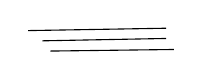
\begin{tikzpicture}
\draw (0,0)--(1.75,.03);
\draw (.18,-.13)--(1.75,-.10);
\draw (.28,-.26)--(1.85,-.24);
\end{tikzpicture}}

\deleted{\unsure{Al|A|II}}

\uline{Globalisation} $\deleted{\unsure{S}}X$ schéma de car. 0, $\theta$ \deleted{\unsure{la|$S$}} dérivation de $\underline O_X$, supposons $\theta$ loc nilpotente. Alors $\exp\theta$ est un autom de $\underline O_X$ qui induit \deleted{\unsure{la}}l'identité sur $\underline O_{X_{\mathrm{réd}}}=\underline O_X/N\underline O_X$, et correspond \unsure{:|à} un autom de $X$ que nous désignons par $\deleted{\unsure{D|E}}\mathbb E_\theta$. Si $\deleted{D} X$ est sur $S$ et $\theta$ est une $S$-dérivation, $\unsure{\epsilon|E}_\theta$ est un $S$-autom. \unsure{Bien.|Enfin.}
\[
\left\{\begin{aligned}
\mathbb E_0&=\mathrm{id}\\
\mathbb E_{\theta+\theta'}&=\deleted{D}\mathbb E_\theta+\mathbb E_{\theta'}\qquad\text{si }[\theta,\theta']=0
\end{aligned}\right.
\]
% archive sheet number: 43
